% ==============================================================================
% LAB 117
% SIMULERING PÅ ELEKTRISKA KRETSAR
% --------------------------------
% Last updated <2015-02-22>
%
% Author:
% Jonas Sjöberg     <tel12jsg@student.hig.se>
% Oscar Wallberg    <tco13owg@student.hig.se>
%
% License:
% Creative Commons Attribution-NonCommercial-ShareAlike 4.0 International
% See LICENSE.md for full licensing information.
% ==============================================================================

% ==============================================================================
% INCLUDES AND CONFIGURATION
% ==============================================================================
\documentclass[11pt,a4paper]{article}
\usepackage[utf8]{inputenc}
\usepackage[swedish]{babel} % För svensk innehållsförteckning
\usepackage{siunitx} % (För dokumentation, kör i terminalen; texdoc siunitx)
\usepackage{amssymb}
\usepackage{amsmath}
\usepackage{amsfonts}
\usepackage{graphicx}
\usepackage{booktabs}
\usepackage{longtable} % Tables span across pages
\usepackage{microtype}
\usepackage{gensymb}
%\usepackage{tabto}
\usepackage{units}
%\usepackage[]{biblatex}
%\addbibresource{bibliografi.bib}
%\bibliography{bibliografi.bib}
%\bibliographystyle{ieeetr}
\usepackage{float}

\setlength\parindent{0pt} % Removes all indentation from paragraphs

% ==============================================================================
% DOCUMENT METADATA
% ==============================================================================
\title{EE466 \\ Lab 117 \\ Simulering på elektriska kretsar}

\author{\\
  Jonas Sjöberg\\
  Högskolan i Gävle,\\
  Elektronikingenjörsprogrammet,\\
  \texttt{tel12jsg@student.hig.se}\\
  \\
  Oscar Wallberg\\
  Högskolan i Gävle,\\
  Dataingenjörsprogrammet,\\
  \texttt{tco13owg@student.hig.se}\\}

\date{}
% ==============================================================================
\begin{document}
% ==============================================================================
\maketitle

\begin{center}
    \begin{tabular}{l r}
        Lab utförd: & ? Februari 2015 \\
        Instruktör: & Efrain Zenteno
    \end{tabular}
\end{center}

% ==============================================================================
% ABSTRACT
% ==============================================================================
\begin{abstract}
    Syftet med laborationen är att genom använda ett simuleringsverktyg pröva
    några av de grundläggande sambanden och satserna i likströmsläran, samt att
    förstå enkla växelströmskretsar. Dessutom bör studenten efter genomförd
    laboration få en förståelse för hur enklare kretsar kan simuleras.
\end{abstract}

\newpage

{
    %\hypersetup{linkcolor=black}
    \setcounter{tocdepth}{3}
    \tableofcontents
}

\newpage

% ==============================================================================
% SECTION: INTRODUKTION
% ==============================================================================
\section{Introduktion}\label{setup}
% ==============================================================================
En uppsättning vanligt förekommande kopplingar och kretsar ska simuleras i
programmet Multisim av National Instruments. Multisim utgör en del av en uppsättning program
för allehanda EDA, t.ex. CAD, PCB-design och simulering, under proprietär och
komersiell licens. Multisim är en variant av simuleringsprogrammet spice som
utvecklades vid "Electronics Research Laboratory of the University of
California, Berkeley". Spice har kommit att bli de facto standard inom
industrin och många verktyg är baserade på någon version av spice.

All uppkoppling görs i ett grafiskt användarinterface, delvis med hjälp av
virtuella mätinstrument men framförallt med den grundläggande funktionaliteten
som återfinns i enklare spice-liknande program.


% ==============================================================================
% SECTION: 1 MÄTNING PÅ SERIESKRETS
% ==============================================================================
\section{Mätning på seriekrets}\label{}
% ==============================================================================
Seriekretsen enligt figur 1 kopplades upp i Multisim. \unit[10]{\si{\volt}}
valdes för spänningskällan.
Motstånden och spänningskällan är ideala och saknar helt simulering av parasitiska
egenskaper som kan beskrivas som t.ex. en seriell induktans och parallell kapacitans.
\cite{ednarticle}

\par I en seriekrets flyter samma ström genom alla punkter. Vi ser att samtliga probar
mäter att strömmen \textbf{I} = \unit[31,3]{\si{\mA}} vilket stämmer.

\begin{figure}[htbp]
    \centering
%        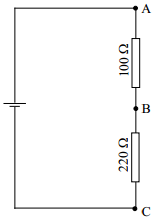
\includegraphics[scale=0.7]{multi/krets1.png}
    \caption{Seriekrets}
    \label{fig:1-mm-schem}
\end{figure}


\subsection{Mätresultat}\label{}
% ------------------------------------------------------------------------------
För att mäta spänningarna vid punkt A, B samt C så placerades prober ut på de
nät som sökts. Proben justeras till att visa relevanta storheter, spänning och
ström.
Spänningarna vid och strömmarna genom alla prober visas i realtid enligt
Figur \ref{fig:sim2}.

\begin{figure}[htbp]
    \centering
    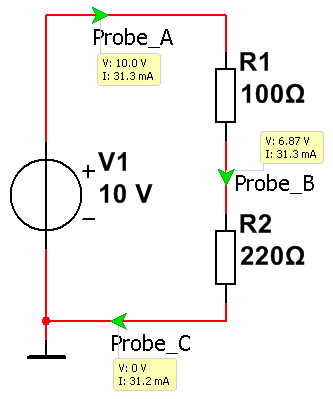
\includegraphics[scale=0.5]{ee466multisim/1.png}
    \caption{Seriekrets}
    \label{fig:sim2}
\end{figure}

För en relativ mätning används \emph{DC operating point}. De sökta spänningarna
beskrivs som skillnaden mellan proberna \textbf{Probe\_A}, \textbf{Probe\_B} och
\textbf{Probe\_C}. Se figur \ref{fig:sim2op} för resultat.

\begin{figure}[htbp]
    \centering
    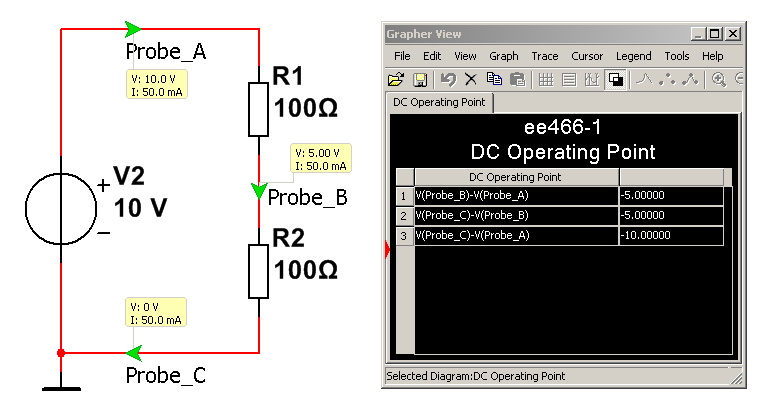
\includegraphics[scale=0.5]{ee466multisim/1-op.png}
    \caption{Simuleringsresultat för seriekrets}
    \label{fig:sim2op}
\end{figure}


\subsection{Kommentar}\label{}
% ------------------------------------------------------------------------------
% TODO: * Kommentera utgående från Kirchhoffs 2:a lag.
%       * Kommentera utgående från spänningsdelningslagen.

Spänningsdelningslagen ger:\\[+2mm]
\begin{math}
U_{AB} = U\times\frac{R_{1}}{R_{1}+R_{2}}\\[+2mm]
U_{AB} = 10\times\frac{100}{100+220}\\[+2mm]
U_{AB} = 3.125\\
\\
U_{BC} = U\times\frac{R_{2}}{R_{1}+R_{2}}\\[+2mm]
U_{BC} = 10\times\frac{220}{100+220}\\[+2mm]
U_{BC} = 6.875\\
\\
\end{math}

Kirchhoff's 2:a lag:

\begin{quote}
Summan av samtliga emk:s som ingår i en sluten krets är lika med summan av potentialfallen, eller\\
\begin{math}
u_{1} + u_{2} + \ldots + u_{n} = 0\\
\text{där }u_{k} \text{ betecknar en potentialändring.}
\end{math}

\end{quote}

Enligt Kirchhoff's lag:\\

$U - U_{AB} - U_{BC} = 0$\\
$10 - 3.125 - 6.875 = 0$, vilket stämmer.

\clearpage

% ==============================================================================
% SECTION: 2 iNVERKAN AV EN PARALLELLGREN PÅ EN KRETS
% ==============================================================================
\section{Inverkan av en parallellgren på en krets}\label{}
% ==============================================================================
Ytterligare en resistor på 330 \si{\ohm} kopplades parallellt till kretsen från
figur \ref{fig:1-mm-schem}, se figur \ref{fig:2-mm-schem}.

\begin{figure}[htbp]
    \centering
        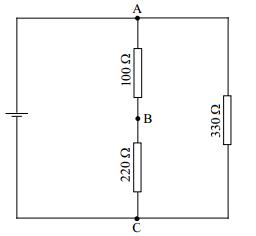
\includegraphics[scale=1.0]{misc/krets2.png}
    \caption{Parallellgren på föregående krets.}
    \label{fig:2-mm-schem}
\end{figure}

\subsection{Mätresultat}\label{}
% ------------------------------------------------------------------------------
Mätresultatet utläses vid proberna i Figur \ref{fig:sim-para}.


\begin{figure}[htbp]
    \centering
    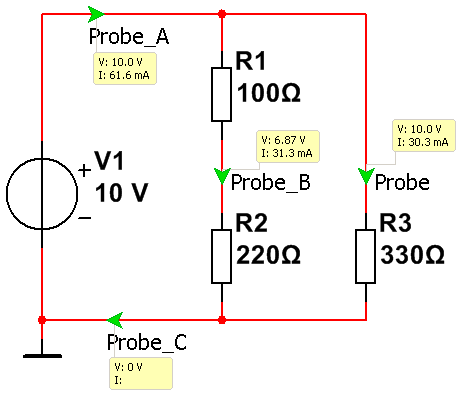
\includegraphics[scale=0.5]{ee466multisim/2.png}
    \caption{Simuleringsresultat för seriekrets med parallellgren.}
    \label{fig:sim-para}
\end{figure}

\clearpage

% ==============================================================================
% SECTION: 3 MÄTNING PÅ PARALLELLKRETS
% ==============================================================================
\section{Mätning på parallellkrets}\label{}
% ==============================================================================
Två resistorer kopplades enligt figur \ref{fig:3-mm-schem}.
Sedan valdes en lämplig spänning för spänningskällan.

\begin{figure}[htbp]
    \centering
        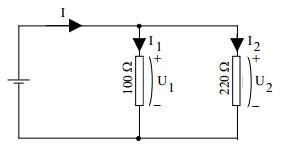
\includegraphics[scale=1]{misc/krets3.png}
    \caption{Parallellgren på föregående krets.}
    \label{fig:3-mm-schem}
\end{figure}

\subsection{Mätresultat}\label{}
% ------------------------------------------------------------------------------
Mätresultat utläses direkt ur Figur \ref{fig:sim3}.

\begin{figure}[htbp]
    \centering
    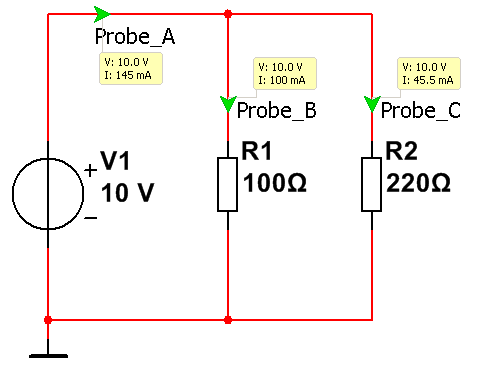
\includegraphics[scale=0.5]{ee466multisim/3.png}
    \caption{Simuleringsresultat för parallellkrets.}
    \label{fig:sim3}
\end{figure}

\subsection{Kommentar}\label{}
% ------------------------------------------------------------------------------
% TODO: Kommentera utgående från Kirchhoffs 1:a lag.
Kirchhoff's 1:a lag:
\begin{quote}
Summan av alla elektriska strömmar som flyter till en nod är lika med summan av alla strömmar som flyter från noden, eller\\
$i_1 + i_2 \ldots + i_n = 0$\\
där $i_k$ betecknar en nodström.
\end{quote}
Detta ger att \\
$I = I_1 + I_2 =
= 0.1 + 0.0455 = 0.1455 \si{\ampere}$\\
Det är möjligt att Probe\_A inte angett fullständig noggrannhet och därav missat en sista decimal. Detta kan förklara varför $I$ inte är detsamma i figur \ref{fig:sim3}.
\clearpage

% ==============================================================================
% SECTION: 4 MÄTNING AV RESISTANS
% ==============================================================================
\section{Mätning av resistans}\label{}
% ==============================================================================
Kretsarna funna i figur \ref{fig:4-mm-schem} kopplades upp.

\begin{figure}[htbp]
    \centering
        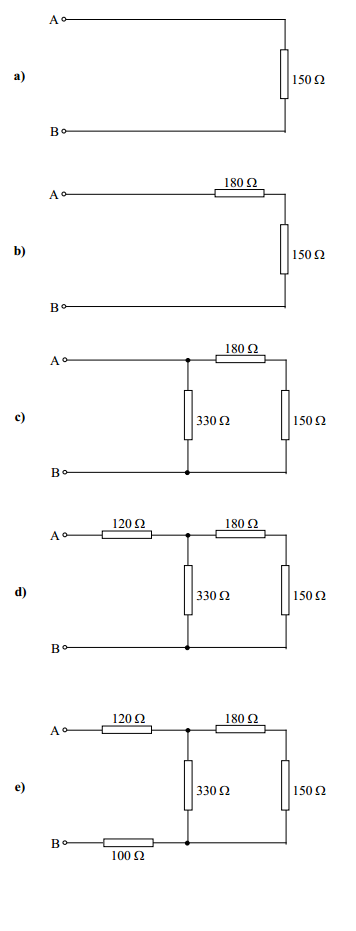
\includegraphics[scale=0.9]{misc/krets4.png}
    \caption{Resistorkretsar.}
    \label{fig:4-mm-schem}
\end{figure}

\subsection{Mätresultat}\label{}
% ------------------------------------------------------------------------------

\subsubsection{A}
\begin{figure}[H]
    \centering
    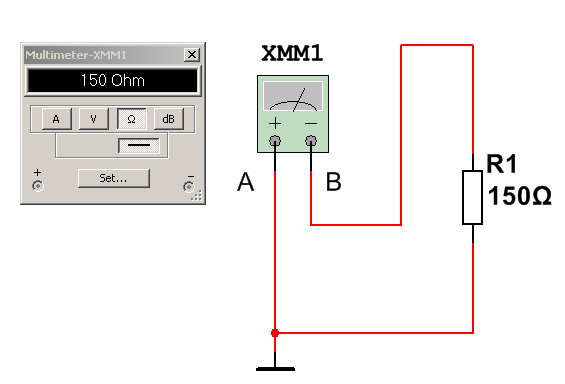
\includegraphics[scale=0.5]{ee466multisim/4a.png}
    \caption{Mätning av resistans A}
    \label{fig:sim-4a}
\end{figure}

\subsubsection{B}
\begin{figure}[H]
    \centering
    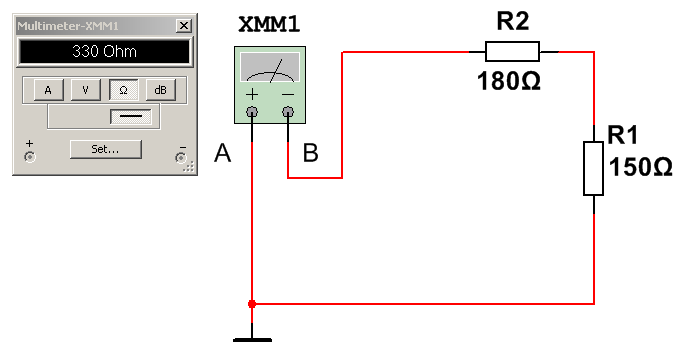
\includegraphics[scale=0.5]{ee466multisim/4b.png}
    \caption{Mätning av resistans B}
    \label{fig:sim-4b}
\end{figure}

\subsubsection{C}
\begin{figure}[H]
    \centering
    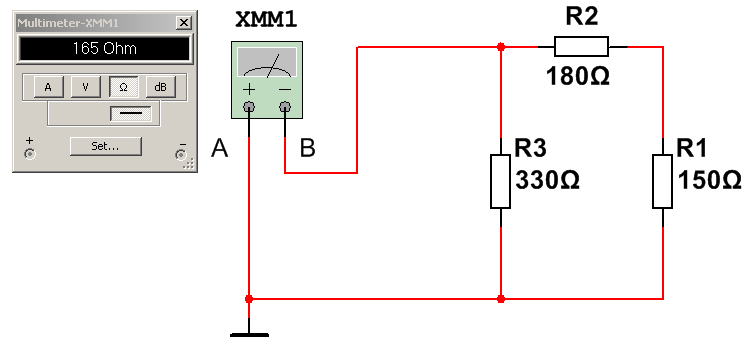
\includegraphics[scale=0.5]{ee466multisim/4c.png}
    \caption{Mätning av resistans C}
    \label{fig:sim-4c}
\end{figure}

\subsubsection{D}
\begin{figure}[H]
    \centering
    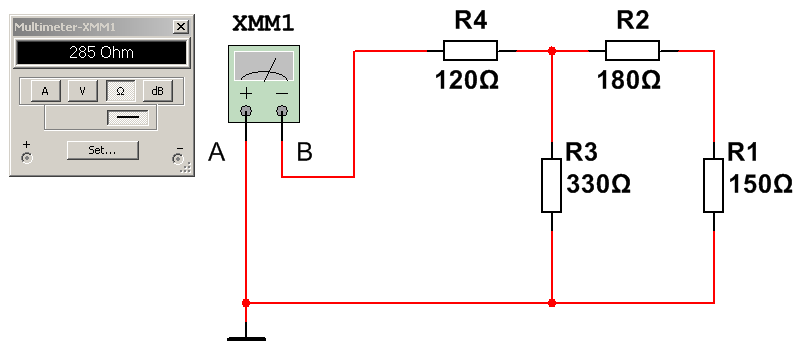
\includegraphics[scale=0.5]{ee466multisim/4d.png}
    \caption{Mätning av resistans D}
    \label{fig:sim-4d}
\end{figure}

\subsubsection{E}
\begin{figure}[H]
    \centering
    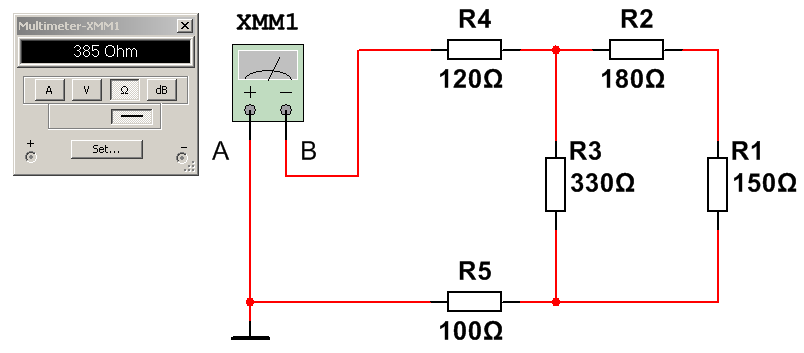
\includegraphics[scale=0.5]{ee466multisim/4e.png}
    \caption{Mätning av resistans E}
    \label{fig:sim-4e}
\end{figure}


\subsection{Teoretisk beräkning}\label{}
% ------------------------------------------------------------------------------
\subsubsection{A}
Resistansen $R_A$ i Figur \ref{fig:sim-4a} utgörs av ett enda motstånd och kan utläsas
direkt till $R_{A} = R_{1} = $\unit[150]{\ohm}

\subsubsection{B}
Resistansen $R_{B}$ i Figur \ref{fig:sim-4b} är teoretiskt;
% 180+150 = 330
\begin{align*}
R_{B}    &= R_{1} + R_{2}                        \\
         &= \unit[150]{\ohm} + \unit[180]{\ohm}  \\
         &= \unit[330]{\ohm}                     \\
\end{align*}

\subsubsection{C}
Resistansen $R_{C}$ i Figur \ref{fig:sim-4c} är teoretiskt;
% 1/((1/330)+(1/(180+150))) = 165
\begin{align*}
R_{C}   &= \frac{1}{\frac{1}{R_{3}} + \frac{1}{R_{1} + R_{2}}} \\
        &= \frac{1}{\frac{1}{330\unit{\ohm}} + \frac{1}{\unit[150]{\ohm} + \unit[180]{\ohm}}} \\
        &= \unit[165]{\ohm}
\end{align*}

\subsubsection{D}
Resistansen $R_{D}$ i Figur \ref{fig:sim-4d} är teoretiskt;
% 1/((1/330)+(1/(180+150)))+120 = 285
\begin{align*}
R_{C}   &= \frac{1}{\frac{1}{R_{3}} + \frac{1}{R_{1} + R_{2}}} + R_{4} \\
&= \frac{1}{\frac{1}{330\unit{\ohm}} + \frac{1}{\unit[150]{\ohm} + \unit[180]{\ohm}}} + \unit[120]{\ohm} \\
&= \unit[285]{\ohm}
\end{align*}

\subsubsection{E}
Resistansen $R_{E}$ i Figur \ref{fig:sim-4e} är teoretiskt;
% 1/((1/330)+(1/(180+150)))+120+100 = 385
\begin{align*}
R_{C}   &= \frac{1}{\frac{1}{R_{3}} + \frac{1}{R_{1} + R_{2}}} + R_{4} + R_{5} \\
&= \frac{1}{\frac{1}{330\unit{\ohm}} + \frac{1}{\unit[150]{\ohm} + \unit[180]{\ohm}}} + \unit[120]{\ohm} + \unit[100]{\ohm}\\
&= \unit[385]{\ohm}
\end{align*}


\subsection{Kommentar}\label{}
% ------------------------------------------------------------------------------
De teoretiska beräkningarna överensstämmer med simuleringen.

\clearpage

% ==============================================================================
% SECTION: 5 STUDIUM AV FREKVENSGÅNG I EN REAKTIV KRETS
% ==============================================================================
\section{Studium av frekvensgång i en reaktiv krets}\label{}
% ==============================================================================
Vid mätning av frekvensgången i en reaktiv krets används kopplingen i Figur
\ref{fig:sim-5-ACanalysis-setup}. Signalgeneratorn kopplas över både resistorn
$R_{1}$ och kondensatorn $C_{1}$ och kan ses som en insignal. Den påverkade
signalen ligger över $C_{1}$, högre frekvenser dämpas mer än lägre frekvenser,
kopplingen utgör ett lågpassfilter.

\subsection{Mätresultat}\label{}
% ------------------------------------------------------------------------------
% TODO: + Gör upp en tabell som för varje frekvens anger
%         - tongeneratorns signalamplitud,
%         - amplituden hos spänningen över den studerade kondensatorn
%         - kvoten mellan den senare amplituden och den tidigare
%         - samt om fasförskjutning förekommer.
% \begin{longtable}[c]{@{}ccc@{}}
%     \toprule\addlinespace
%     \begin{tabular}{ll}Frekvens
%     \end{tabular} & \begin{tabular}{ll}$V_{in}$
% \end{tabular} & \begin{tabular}{ll}$V_{ut}$
% \end{tabular}
% \\\addlinespace
% \midrule\endhead
% 100\si{\Hz} & 1 \si{\volt} & 1,01 \si{\kilo\hertz}
% \\\addlinespace
% 300\si{\Hz} & 1 \si{\volt} & 1,01 \si{\kilo\hertz}
% \\\addlinespace
% 500\si{\Hz} & 1 \si{\volt} & 1,009 \si{\kilo\hertz}
% \\\addlinespace
% 700\si{\Hz} & 1 \si{\volt} & 1,009 \si{\kilo\hertz}
% \\\addlinespace
% 900\si{\Hz} & 1 \si{\volt} & 1,009 \si{\kilo\hertz}
% \\\addlinespace
% 1,10\si{\kHz} & 1 \si{\volt} & 1,009 \si{\kilo\hertz}
% \\\addlinespace
% 1,30\si{\kHz} & 1 \si{\volt} & 1,009 \si{\kilo\hertz}
% \\\addlinespace
% 1,50\si{\kHz} & 1 \si{\volt} & 1,009 \si{\kilo\hertz}
% \\\addlinespace
% 1,70\si{\kHz} & 1 \si{\volt} & 1,009 \si{\kilo\hertz}
% \\\addlinespace
% 1,90\si{\kHz} & 1 \si{\volt} & 1,009 \si{\kilo\hertz}
% \\\addlinespace
% \bottomrule
% \addlinespace
% \caption{Jämförelse av olika kurvformer.}
% \label{vdivtable2}
% \end{longtable}


\subsubsection{Oscilloskopsvy}
\begin{figure}[H]
    \centering
    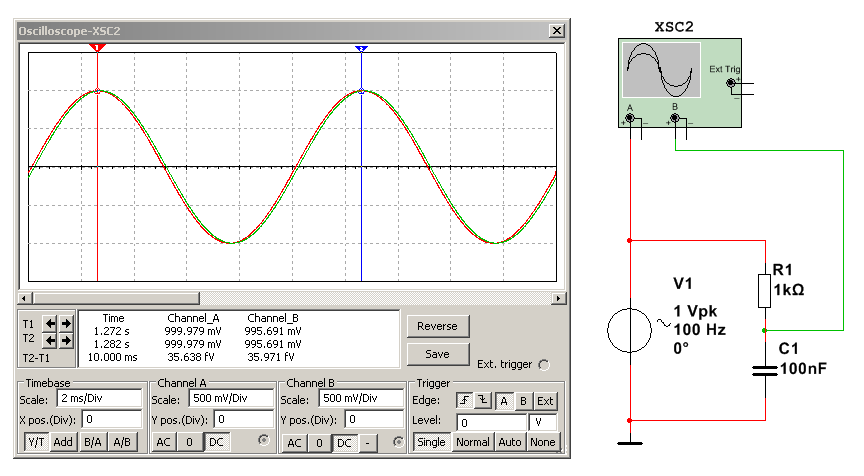
\includegraphics[scale=0.5]{ee466multisim/5-100Hz.png}
    \caption{Signalfrekvens 100Hz}
    \label{fig:sim-5-100Hz}
\end{figure}

\begin{figure}[H]
    \centering
    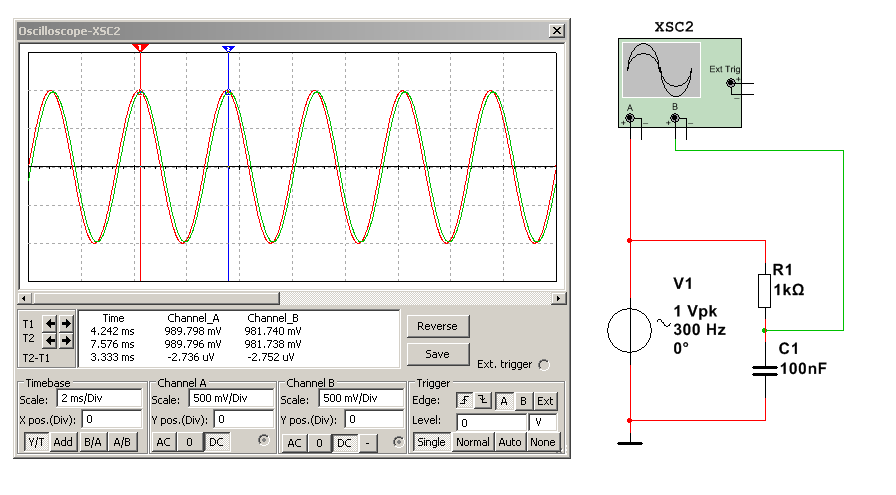
\includegraphics[scale=0.5]{ee466multisim/5-300Hz.png}
    \caption{Signalfrekvens 300Hz}
    \label{fig:sim-5-300Hz}
\end{figure}

\begin{figure}[H]
    \centering
    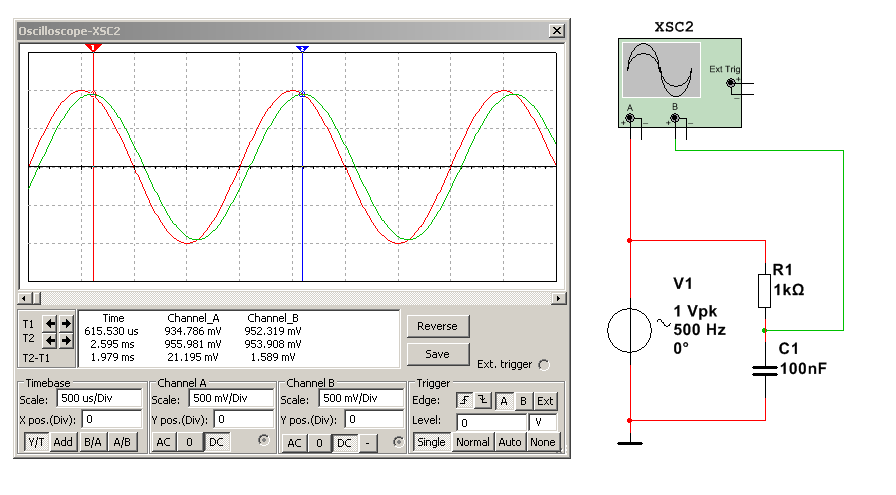
\includegraphics[scale=0.5]{ee466multisim/5-500Hz.png}
    \caption{Signalfrekvens 500Hz}
    \label{fig:sim-5-500Hz}
\end{figure}

\begin{figure}[H]
    \centering
    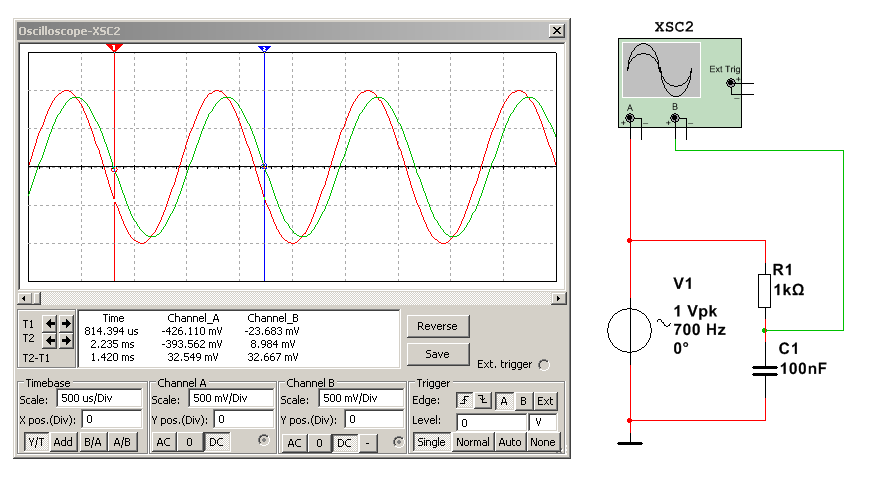
\includegraphics[scale=0.5]{ee466multisim/5-700Hz.png}
    \caption{Signalfrekvens 700Hz}
    \label{fig:sim-5-700Hz}
\end{figure}

\begin{figure}[H]
    \centering
    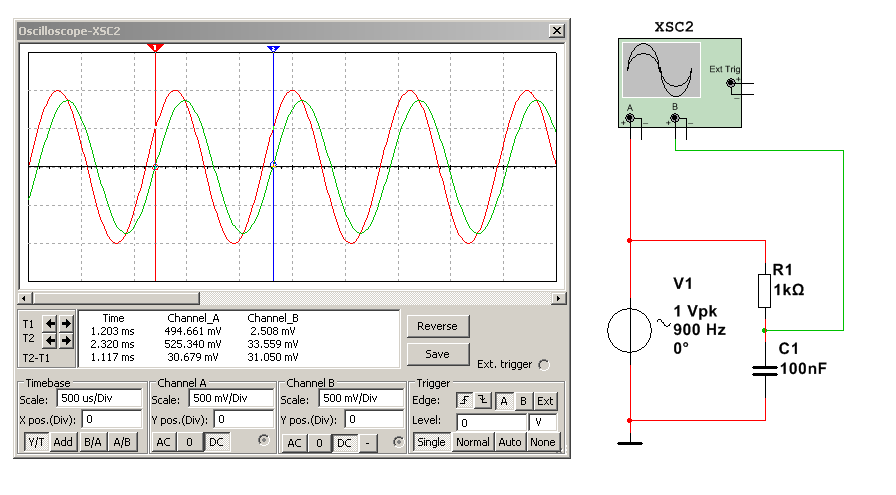
\includegraphics[scale=0.5]{ee466multisim/5-900Hz.png}
    \caption{Signalfrekvens 900Hz}
    \label{fig:sim-5-900Hz}
\end{figure}

\begin{figure}[H]
    \centering
    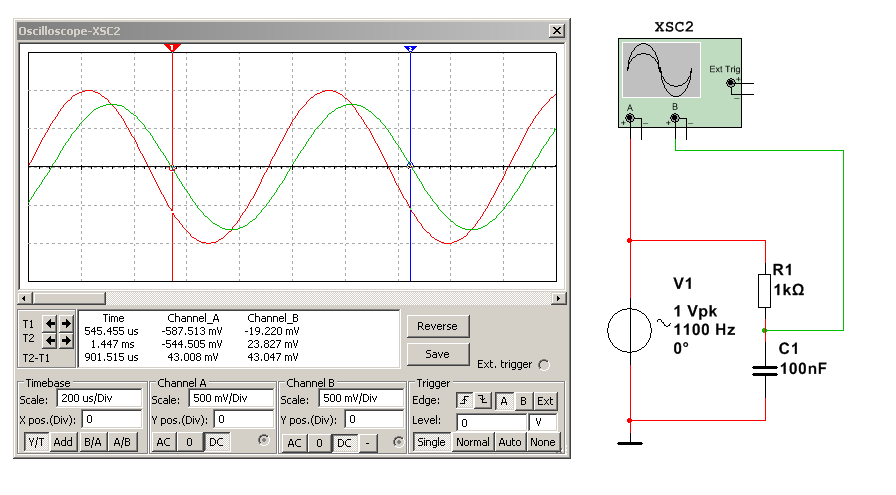
\includegraphics[scale=0.5]{ee466multisim/5-1100Hz.png}
    \caption{Signalfrekvens 1100Hz}
    \label{fig:sim-5-1100Hz}
\end{figure}

\begin{figure}[H]
    \centering
    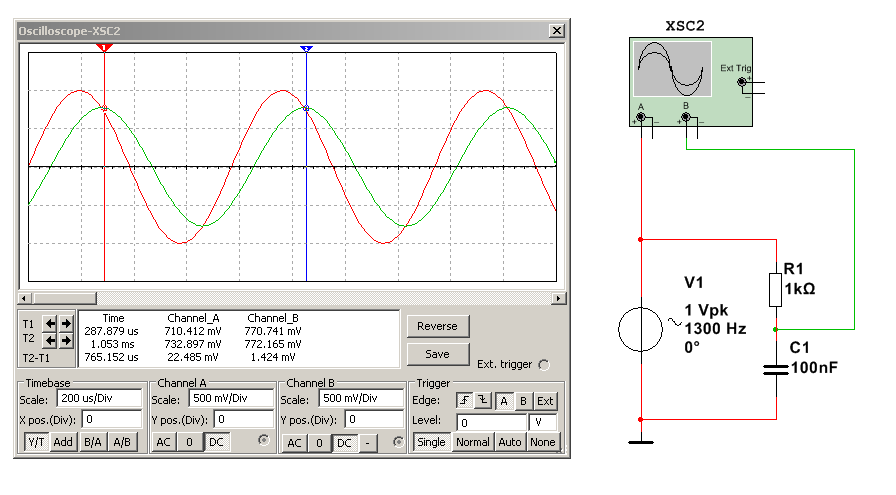
\includegraphics[scale=0.5]{ee466multisim/5-1300Hz.png}
    \caption{Signalfrekvens 1300Hz}
    \label{fig:sim-5-1300Hz}
\end{figure}

\begin{figure}[H]
    \centering
    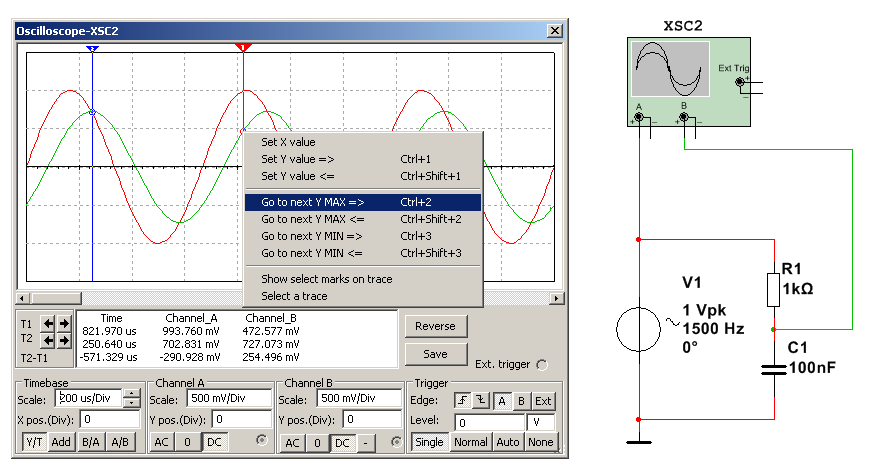
\includegraphics[scale=0.5]{ee466multisim/5-1500Hz.png}
    \caption{Signalfrekvens 1500Hz}
    \label{fig:sim-5-1500Hz}
\end{figure}

\begin{figure}[H]
    \centering
    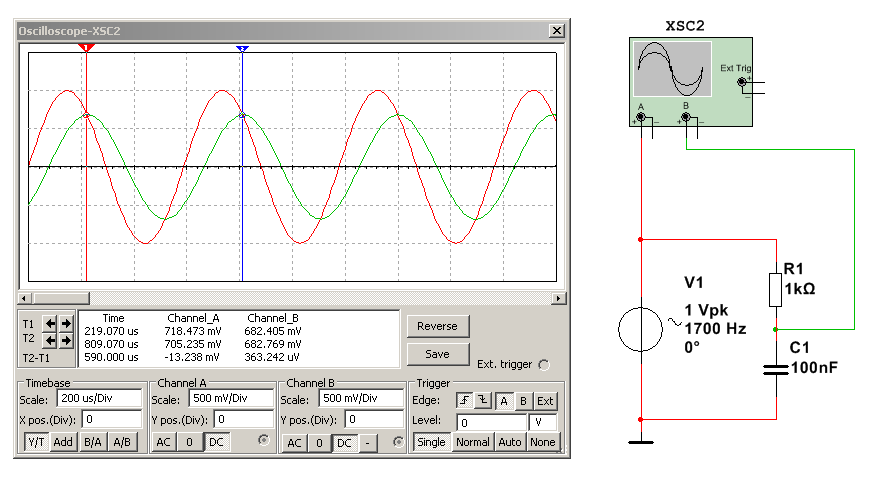
\includegraphics[scale=0.5]{ee466multisim/5-1700Hz.png}
    \caption{Signalfrekvens 1700Hz}
    \label{fig:sim-5-1700Hz}
\end{figure}

\begin{figure}[H]
    \centering
    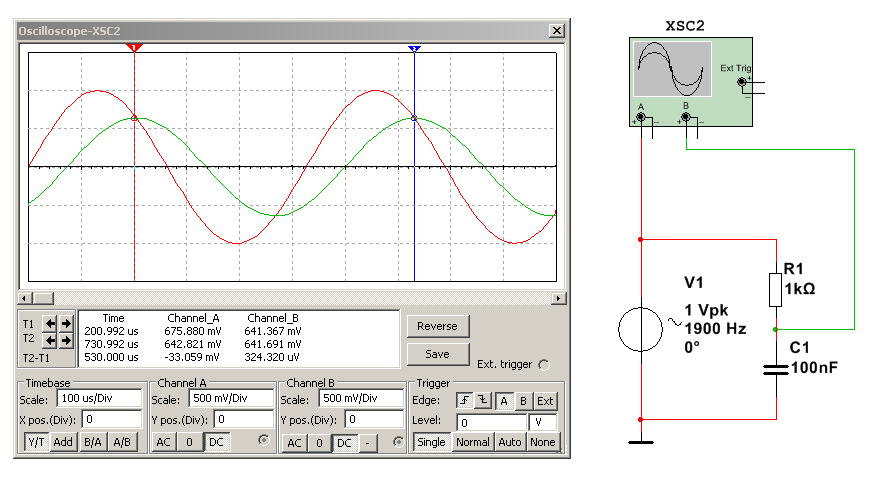
\includegraphics[scale=0.5]{ee466multisim/5-1900Hz.png}
    \caption{Signalfrekvens 1900Hz}
    \label{fig:sim-5-1900Hz}
\end{figure}


\subsubsection{AC analys}
\begin{figure}[htbp]
    \centering
    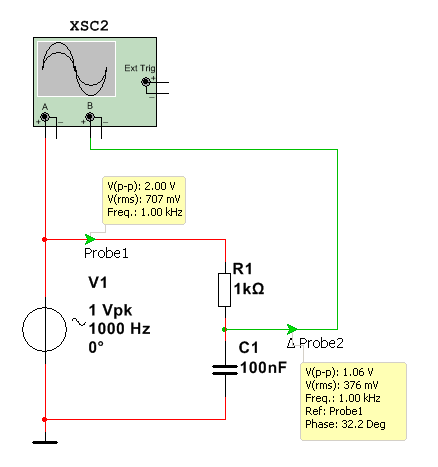
\includegraphics[scale=0.5]{ee466multisim/5-ACprobes.png}
    \caption{Koppling vid AC analys}
    \label{fig:sim-5-ACanalysis-setup}
\end{figure}

\begin{figure}[htbp]
    \centering
    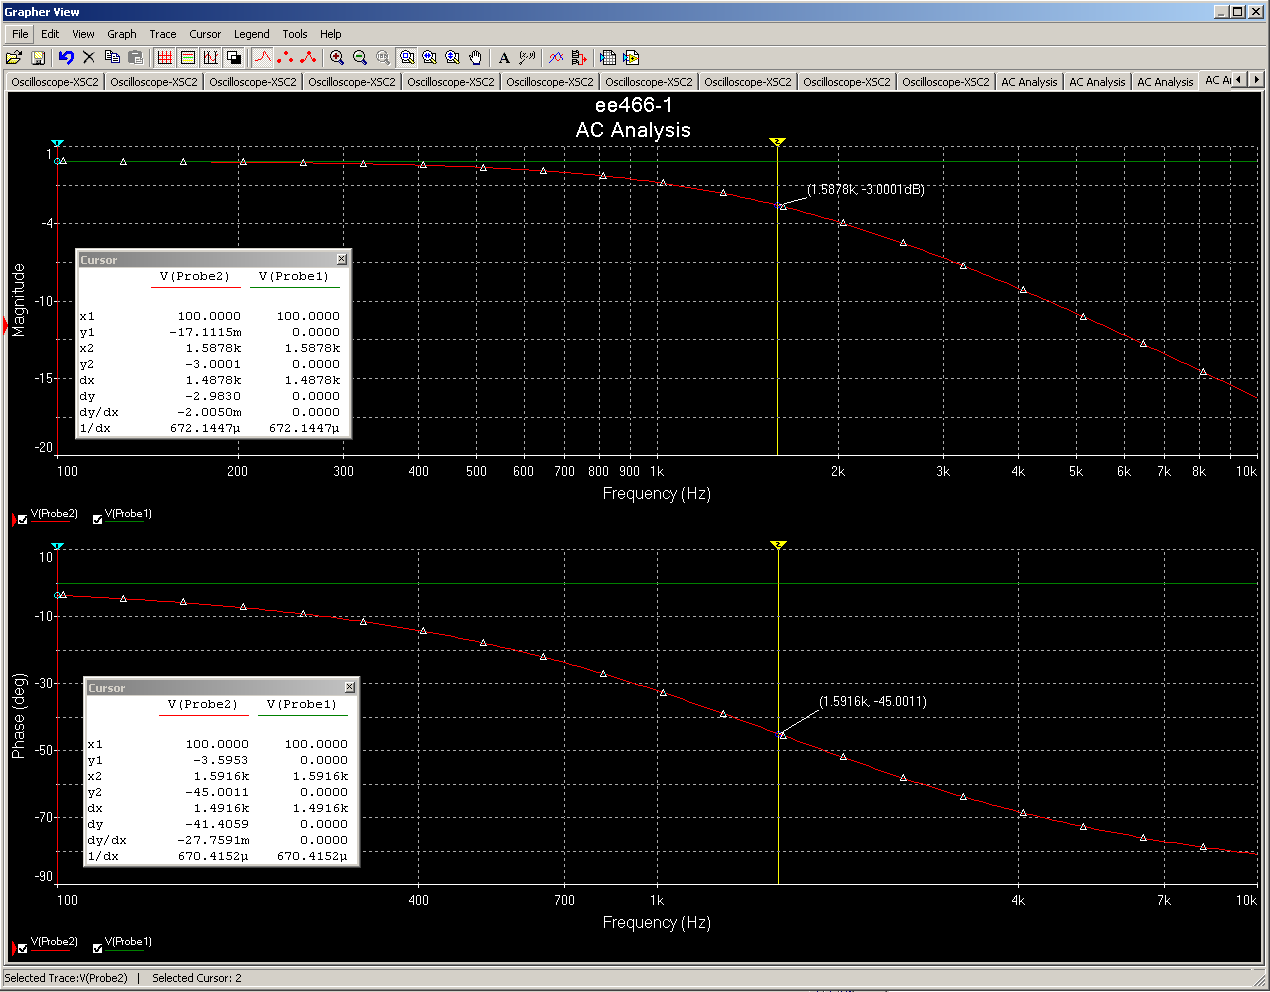
\includegraphics[scale=0.4]{ee466multisim/5-ACanalysis.png}
    \caption{AC analys resultat}
    \label{fig:sim-5-ACanalysis-results}
\end{figure}


\subsection{Teoretisk beräkning}\label{}
% ------------------------------------------------------------------------------
\begin{align*}
%\frac{u_{c}}{u_{TG}} &= \frac{1}{\sqrt{1+(2 \pi \times f \times R \times C)^2}}\\
$A_{v}$ &= \frac{1}{\sqrt{1+(2 \pi \times f \times R \times C)^2}}\\
&= \frac{1}{\sqrt{1 + (2 \pi \times \unit[100]{\Hz} \times 1)}}
%                     &= \frac{1}{\sqrt{1+(2 \pi \times \unit[100]{\Hz} \times \unit[1]{\kohm} \times \unit[100]{\nanofarad}})^2}}\\
%                     &= \frac{1}{\sqrt{1+(2 \pi \times 100 \times \num{1e3} \times \num{100e-9})^2}}
\end{align*}


\subsection{Kommentar}\label{}
% ------------------------------------------------------------------------------
% TODO:

\clearpage

% ==============================================================================
% SECTION: 6 MÄTNING AV FASFÖRSKJUTNING I EN REAKTIV KRETS
% ==============================================================================
\section{Mätning av fasförskjutning i en reaktiv krets}\label{}
% ==============================================================================
Vi mätningen av fasförskjutning används samma simuleringskonfiguration som vid
föregående mätning.

\subsection{Mätresultat}\label{}
% ------------------------------------------------------------------------------
Signalens fas utläses ur den nedre grafen i Figur \ref{fig:sim-5-ACanalysis-results}.

\subsection{Teoretisk beräkning}\label{}
% ------------------------------------------------------------------------------
% TODO: Kontrollera dina resultat genom att utnyttja följande formel: ϕ = −arctan(2π ⋅f ⋅R ⋅C) 
Formeln\\
	$\phi = -arctan(2\times \pi\times f\times R\times C)$\\
ger\\
$ -arctan(2\times \pi\times 1591.6\times 1000\times 100\times 10^-9) = -45.00091$\\
vilket stämmer enligt figur \ref{fig:sim-5-ACanalysis-results}.

\subsection{Kommentar}\label{}
% ------------------------------------------------------------------------------
% TODO: Kommentera resultatet
Det är tänkbart att AC-analysen beräknar resultatet med fler värdesiffror på frekvensen än vad som anges i grafen, vilket resulterar i en liten skillnad i decimalerna jämfört med den teoretiska beräkningen.
\clearpage

% ==============================================================================
% SECTION: 7 MÄTNING AV RESONANSFREKVENS
% ==============================================================================
\section{Mätning av resonansfrekvens}\label{}
% ==============================================================================
% TODO: Kopplingsschema.

\subsection{Mätresultat}\label{}
% ------------------------------------------------------------------------------
Simuleringsresultatet för AC-analysen visas i Figur \ref{fig:7-ACanalysis}.
Signalkällans frekvens sveps mellan \unit[100]{\si{\Hz}}-\unit[100]{\si{\kHz}}.
Amplituden utläses vertikalt och har enheten \si{\dB}, vilket är lämpligt för
att visa små förändringar över ett stort intervall.
\par I den övre grafen är den gula markören positionerad vid resonansfrekvensen
som utläses under \textbf{Probe2}, $F_{resonans} = $\unit[15,8489]{\si{\kHz}}.
Den nedre grafen visar fasförskjutningen som vid resonansfrekvensen närmar sig noll.


\begin{figure}
    \centering
    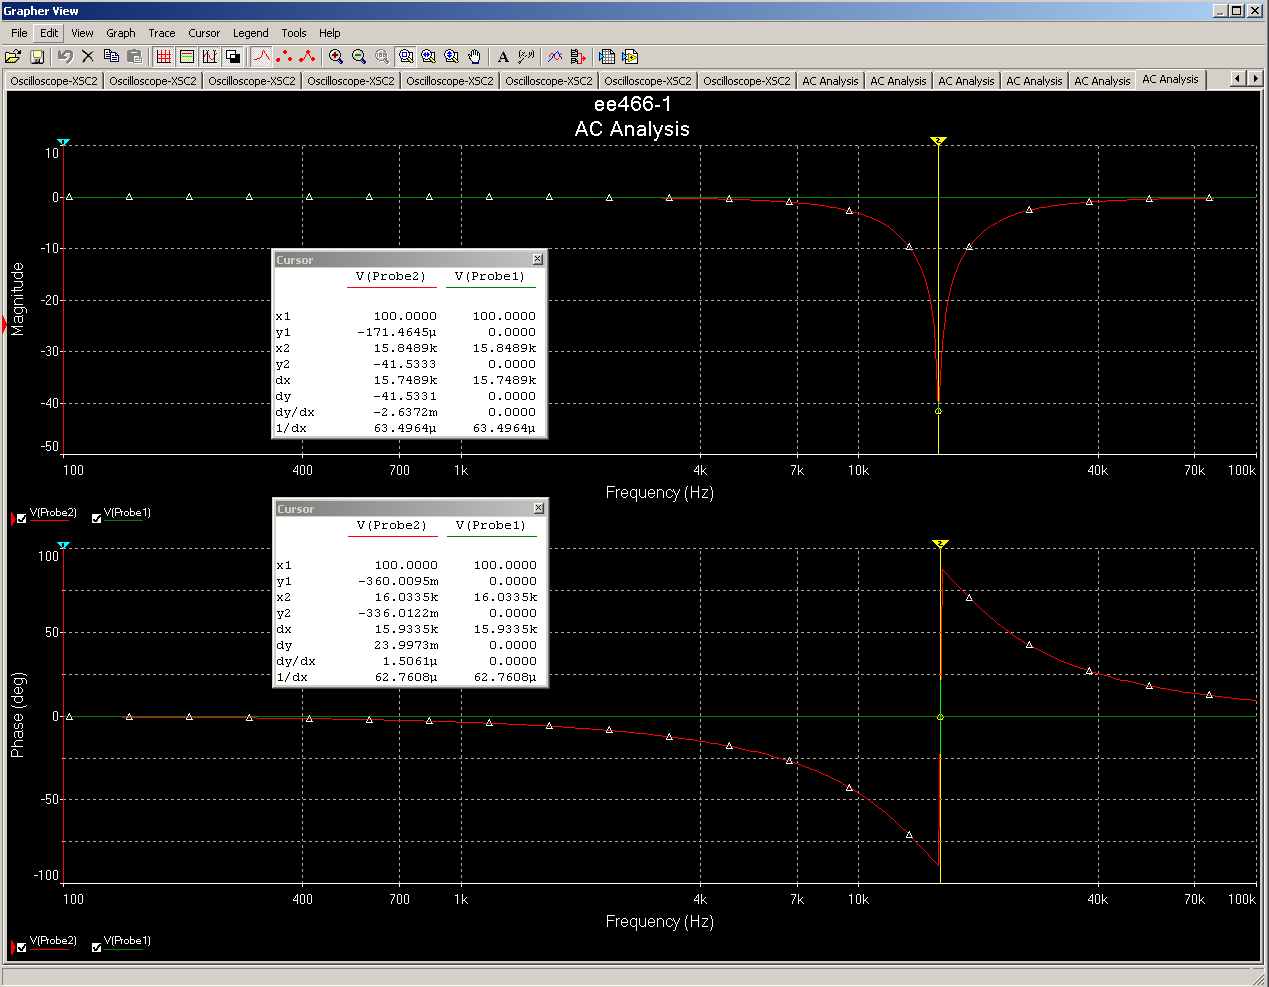
\includegraphics[width=1.25\linewidth]{ee466multisim/7-ACanalysis}
    \caption{Resonansfrekvens AC analys resultat}
    \label{fig:7-ACanalysis}
\end{figure}



\subsection{Kommentar}\label{}
% ------------------------------------------------------------------------------
% TODO: + Kommentera följande:
%         - Förekommer fasförskjutning mellan uTG och uR vid denna frekvens?
%         - Ändrar fasen sig om du varierar frekvensen kring den
%           uppmätta resonansfrekvensen?  I så fall hur?
%         - Om laboration 61 har gjorts, jämför resultatet med de uppmätta
%           värderna.  Stämmer de överens om inte, varför?


% ==============================================================================
% SECTION: RESULTAT
% ==============================================================================
\section{Resultat}\label{setup}
% ==============================================================================
% TODO: Övergripande resultat/sammanfattning/kommentar på HELA labben.

\newpage

% ==============================================================================
% SECTION: REFERENSER
% ==============================================================================
\section{Referenser}\label{refs}
% ==============================================================================
% TODO: Referenser.

\textbf{Resistors aren't resistors} Wyatt, Kenneth. \textit{EDN Magazine 2013-10-29}
\texttt{www.edn.com/design/components-and-packaging/4423492/Resistors-aren-t-resistors}



%\printbibliography


%\subsection{Källkod}\label{sourcefiles}
% ------------------------------------------------------------------------------

% ==============================================================================
\end{document}
% ==============================================================================
